\documentclass[conference]{IEEEtran}

\usepackage[utf8]{inputenc}
\usepackage[T1]{fontenc}
\usepackage{amsmath,amssymb}
\usepackage{graphicx}
\usepackage{booktabs}
\usepackage{algorithm}
\usepackage{algpseudocode}
\usepackage{hyperref}
\usepackage{cite}
\usepackage{xcolor}
\usepackage{subcaption}
\usepackage{multirow}
\usepackage{float}
\usepackage{balance}
\usepackage{tikz}
\usetikzlibrary{shapes,arrows.meta,positioning,fit,calc}

\hypersetup{colorlinks=false}

\title{Multi-Agent Reinforcement Learning for Adaptive Data Rate Optimization in Dense LoRaWAN Networks}

\author{
\IEEEauthorblockN{N.N.D. Perera, R.T. Thudewattage, D.D.M. Jayasooriya, M.N.Z. Ahamed}
\IEEEauthorblockA{Department of Computer Science and Engineering\\
University of Moratuwa, Sri Lanka\\
\{perera.210476, thudewattage.210652, jayasooriya.210250, ahamed.210023\}@uom.lk}
\and
\IEEEauthorblockN{Uthayasanker Thayasivam}
\IEEEauthorblockA{Department of Computer Science and Engineering\\
University of Moratuwa, Sri Lanka}
\and
\IEEEauthorblockN{Thushan Sivalingam}
\IEEEauthorblockA{Centre for Wireless Communications\\
University of Oulu, Finland}
}

\begin{document}

\maketitle

\begin{abstract}
Dense LoRaWAN deployment for Industry 4.0 application suffer from severe packet loss due to collision and interference. Classical Adaptive Data Rate (ADR) mechanism cannot handle the dynamic, competitive nature of these environment, often achieving below 40\% packet delivery rate (PDR). In this paper, we propose a Multi-Agent Reinforcement Learning (MARL) approach to ADR optimization where each device is represented by an independent agent with coordination signal for channel-aware collision avoidance. We compare MARL against classical ADR, Proximal Policy Optimization (PPO), and Deep Q-Network based approaches across 11 experiment scenario in ns-3, with device count ranging from 10 to 200. Our result show that MARL achieve up to 99.63\% PDR in dense scenario where classical ADR deliver only 42\%, while maintaining comparable energy consumption. In scalability test, MARL degrade more gracefully and achieve 58\% higher Jain's fairness index than single-agent method. We also validate the approach on physical testbed with ESP32 device and SX1278 LoRa module.
\end{abstract}

\begin{IEEEkeywords}
LoRaWAN, Adaptive Data Rate, Multi-Agent Reinforcement Learning, IoT, Deep Q-Network, Packet Delivery Rate
\end{IEEEkeywords}

% ============================================================================
\section{Introduction}
\label{sec:intro}
% ============================================================================

Long Range Wide Area Network (LoRaWAN) have become one of the most adopted Low Power Wide Area Network (LPWAN) technology for Internet of Things (IoT) application, thanks to their long range capability, low power consumption, and cost effectiveness \cite{Raza17, augustin2016study}. LoRaWAN use Chirp Spread Spectrum (CSS) modulation to achieve robustness against interference and multipath fading. However, as deployment density increase to support Industry 4.0 and smart city ecosystem, the limitation of LoRaWAN architecture become apparent.

LoRaWAN employ a Pure ALOHA medium access control where device transmit asynchronously without carrier sensing \cite{georgiou2017low}. While efficient for sparse network, this approach have a theoretical maximum throughput of only 18.4\% channel capacity. In dense scenario with 20 to 200 device transmitting frequently within confined area, the packet delivery rate (PDR) of classical LoRaWAN often collapse to below 40\% \cite{bor2016lora, bankov2016mathematical}.

The classical Adaptive Data Rate (ADR) mechanism attempt to mitigate this by adjusting spreading factor (SF) and transmission power (TP) based on the average SNR of last 20 received packet. However, this reactive, myopic approach have several critical flaw \cite{slabicki2018adaptive}: (1) it lag behind rapidly changing interference condition; (2) it operate on device-by-device basis without global coordination, often causing ``SF convergence'' where multiple device settle on same SF and channel; and (3) it cannot differentiate between collision and noise-induced loss.

Recent work have explored deep learning and reinforcement learning (RL) for ADR optimization. Farhad et al. \cite{farhad2021deep} propose a deep learning-based ADR that use neural network to predict optimal parameter, but it is limited to supervised prediction without adaptive decision-making capability. Ta et al. \cite{ta2023enhanced} propose an enhanced RL-based transmission parameter selection that optimize energy and PDR, but consider only single-agent scenario. Moy et al. \cite{moy2024energy} apply RL to subterranean LoRaWAN for satellite communication and show energy efficiency improvement, but do not address multi-agent coordination needed in dense surface deployment. Yazid et al.~\cite{yazid2022rl} formulate parameter selection as an MDP with tabular Q-learning but evaluate on only 10 device in static environment, making it unclear whether the approach scale to dense deployment. Abdelfadeel et al.~\cite{abdelfadeel2020machine} propose a fair ADR allocation using heuristic SF assignment, yet rely on centralized optimization that assume global knowledge and do not account for dynamic interference or channel-level collision. Reynders et al.~\cite{reynders2018improving} introduce lightweight scheduling to improve scalability but require modification to the LoRaWAN MAC layer and evaluate with at most 15 device, far below practical Industry~4.0 density. None of these work combine multi-agent reinforcement learning with explicit channel coordination or evaluate at scale beyond 30 device.

The key insight of our work is that dense LoRaWAN deployment is not simply an optimization problem but a \textit{competitive game} where each device action (SF, TP, channel choice) directly affect the collision probability of all other device. This multi-agent interaction cannot be captured by single-agent RL or prediction-based method. We propose MARL with coordination signal that enable distributed collision avoidance while keeping the computational overhead manageable.

Our contribution are:
\begin{enumerate}
    \item We formulate dense LoRaWAN ADR as a Markov Game and propose Independent Q-Learning with coordination signal for channel-aware collision avoidance.
    \item We implement and compare MARL against classical ADR, PPO, and DQN-based method across 11 scenario in ns-3 simulator with realistic WiFi and LTE interference.
    \item We conduct first large-scale evaluation (up to 200 device) showing MARL degrade more gracefully with higher Jain's fairness index than single-agent approach.
    \item We validate feasibility on physical testbed with ESP32 and SX1278 LoRa hardware.
\end{enumerate}

% ============================================================================
\section{System Model}
\label{sec:system}
% ============================================================================

\subsection{Problem Formulation}

We consider a LoRaWAN network with $N$ end device communicating with a single gateway operating in the EU868 ISM band with 8 available channel. Each device $i$ periodically transmit packet and must select transmission parameter: spreading factor $\text{SF}_i \in \{7, \ldots, 12\}$, transmission power $\text{TP}_i \in \{8, 11, 14\}$~dBm, and channel $c_i \in \{0, \ldots, 7\}$.

Two packet collide when transmitted on the same channel with the same SF during overlapping time interval. The Time-on-Air (ToA) depend exponentially on SF:
\begin{equation}
    T_{\text{air}} = \frac{N_{\text{sym}}}{B / 2^{\text{SF}}}
\end{equation}
where $B = 125$~kHz is the bandwidth and $N_{\text{sym}}$ is the total symbol count. Higher SF increase ToA and therefore both collision probability and energy consumption.

The energy per transmission is:
\begin{equation}
    E = V \cdot (85 + 2.3(P_{tx} - 2)) \cdot T_{\text{air}} + E_{\text{rx}}
    \label{eq:energy}
\end{equation}
where $V = 3.3$~V is supply voltage, the current model is derived from the SX1278 datasheet \cite{semtech_sx1278}, and $E_{\text{rx}} = 0.033$~mJ is receive window overhead.

\subsection{MDP Formulation}

For single-agent approach (DQN, PPO), the problem is formulated as an MDP $(\mathcal{S}, \mathcal{A}, \mathcal{P}, \mathcal{R}, \gamma)$. The state vector for device $i$ at time $t$:
\begin{align}
    s_t = \big[&\text{RSSI}_n,\, \sigma^2_{\text{RSSI}},\, \text{SNR}_n,\, \Delta\text{SNR},\, \text{PDR}_r,\, \Delta\text{PDR}, \nonumber\\
    &\tfrac{L_c}{5},\, \tfrac{t_i}{300},\, \tfrac{\text{SF}-7}{5},\, \tfrac{\text{TP}-2}{12},\, \tfrac{c}{7}\big]
\end{align}
where $L_c$ is consecutive loss count and $t_i$ is time since last success. All feature are normalized to $[0, 1]$. The action space comprise 48 discrete action combining SF~$\in\{7,\ldots,12\}$, TP~$\in\{8, 11, 14\}$~dBm, and a binary channel-change decision ($2 \times 6 \times 3 = 36$ base action $+ 12$ channel-hop variant). Discount factor $\gamma = 0.95$.

\subsection{Markov Game for MARL}

In dense deployment, each device action affect others through collision. We model this as a Markov Game $(\mathcal{S}, \mathcal{A}_1, \ldots, \mathcal{A}_N, \mathcal{P}, \mathcal{R}_1, \ldots, \mathcal{R}_N, \gamma)$ where the state transition depend on the joint action of all agent.

The MARL state vector extend the local state with a coordination feature:
\begin{equation}
    s_t^{\text{MARL}} = \left[s_t^{\text{local}},\; n_{\text{same\_ch}} / 3\right]
\end{equation}
where $n_{\text{same\_ch}}$ is the count of other device using the same channel, provided through the network server channel tracking map.

\subsection{Congestion-Adaptive Reward}

The reward function dynamically adjust based on estimated congestion level $C \in [0, 1]$:
\begin{equation}
    r_t = w_1 R_{\text{outcome}} + w_2 R_{\text{interference}} + w_3 R_{\text{stability}} + w_4 R_{\text{efficiency}}
\end{equation}
where $w_1 = 0.4 + 0.3(1-C)$, $w_2 = 0.25C$, $w_3 = 0.2 + 0.15(1-C)$, $w_4 = 0.15 + 0.2(1-C)$. The congestion level is estimated from traffic intensity $N/T_{\text{period}}$, pre-TX RSSI, and recent PDR.

% ============================================================================
\section{Proposed Method}
\label{sec:method}
% ============================================================================

\subsection{MARL Agent Architecture}

Fig.~\ref{fig:architecture} illustrate the system architecture. The network server maintain a digital twin RL agent for each end device, a channel tracking map recording current channel assignment, and a coordination signal generator. Uplink metadata (RSSI, SNR, success/failure) update the corresponding digital twin, which select the next action. The selected SF, TP, and channel are communicated to the device via standard LoRaWAN downlink MAC command.

\begin{figure}[t]
\centering
\resizebox{\columnwidth}{!}{%
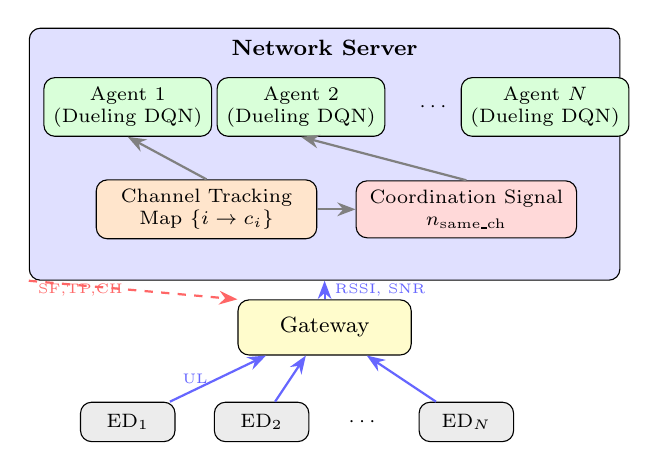
\begin{tikzpicture}[>=Stealth, node distance=0.6cm,
  block/.style={rectangle, draw, rounded corners, minimum height=0.7cm, minimum width=1.8cm, align=center, font=\footnotesize},
  smallblock/.style={rectangle, draw, rounded corners, minimum height=0.5cm, minimum width=1.2cm, align=center, font=\scriptsize},
  arrow/.style={->, thick}]

  % Network Server box
  \node[block, fill=blue!12, minimum width=7.5cm, minimum height=3.2cm] (ns) at (0,2.4) {};
  \node[font=\footnotesize\bfseries] at (0,3.75) {Network Server};

  % Digital Twins
  \node[smallblock, fill=green!15] (dt1) at (-2.5,3.0) {Agent 1\\(Dueling DQN)};
  \node[smallblock, fill=green!15] (dt2) at (-0.3,3.0) {Agent 2\\(Dueling DQN)};
  \node[font=\scriptsize] at (1.4,3.0) {$\cdots$};
  \node[smallblock, fill=green!15] (dtn) at (2.8,3.0) {Agent $N$\\(Dueling DQN)};

  % Channel map and coordination
  \node[smallblock, fill=orange!20, minimum width=2.8cm] (chmap) at (-1.5,1.7) {Channel Tracking\\Map $\{i \to c_i\}$};
  \node[smallblock, fill=red!15, minimum width=2.8cm] (coord) at (1.8,1.7) {Coordination Signal\\$n_{\text{same\_ch}}$};

  % Gateway
  \node[block, fill=yellow!20, minimum width=2.2cm] (gw) at (0,0.2) {Gateway};

  % End Devices
  \node[smallblock, fill=gray!15] (ed1) at (-2.5,-1.0) {ED$_1$};
  \node[smallblock, fill=gray!15] (ed2) at (-0.8,-1.0) {ED$_2$};
  \node[font=\scriptsize] at (0.5,-1.0) {$\cdots$};
  \node[smallblock, fill=gray!15] (edn) at (1.8,-1.0) {ED$_N$};

  % Arrows: uplink
  \draw[arrow, blue!60] (ed1) -- (gw) node[midway, left, font=\tiny] {UL};
  \draw[arrow, blue!60] (ed2) -- (gw);
  \draw[arrow, blue!60] (edn) -- (gw);
  \draw[arrow, blue!60] (gw) -- (ns.south) node[midway, right, font=\tiny] {RSSI, SNR};

  % Arrows: downlink
  \draw[arrow, red!60, dashed] (ns.south west) -- (gw.north west) node[midway, left, font=\tiny] {SF,TP,CH};

  % Internal arrows
  \draw[arrow, gray] (chmap) -- (coord);
  \draw[arrow, gray] (coord.north) -- (dt2.south);
  \draw[arrow, gray] (chmap.north) -- (dt1.south);

\end{tikzpicture}}
\caption{MARL system architecture. The network server host independent digital twin agent for each device, coordinated through a shared channel tracking map.}
\label{fig:architecture}
\end{figure}

Each MARL agent use a Dueling DQN architecture \cite{wang2016dueling} with 12 input feature and 48 output action. The network separate state value estimation from advantage estimation:
\begin{equation}
    Q(s, a) = V(s) + A(s, a) - \frac{1}{|\mathcal{A}|}\sum_{a'} A(s, a')
\end{equation}

The architecture consist of two shared hidden layer (64 unit each with Leaky ReLU), followed by separate value stream and advantage stream (each 32 unit). Training use Prioritized Experience Replay (PER) \cite{schaul2016per} with capacity 20,000, $\alpha = 0.6$, $\beta = 0.4$, and Double DQN target update \cite{van2016deep} every 50 step.

\subsection{Coordination-Aware Action Selection}

The key innovation of our MARL approach is the coordination-aware $\epsilon$-greedy policy. Before standard action selection, each agent check if its current channel is congested:

\begin{algorithm}[t]
\caption{MARL Coordination-Aware Action Selection}
\label{alg:marl}
\begin{algorithmic}[1]
\Require Channel usage map, current channel $c$, $\epsilon$
\State $\text{count}[c] \gets |\{j \neq i : c_j = c\}|$
\If{$\text{count}[c] \geq 2$ \textbf{and} rand() $< 0.4$}
    \State $c^* \gets \arg\min_k \text{count}[k]$
    \State \Return channel-change action for $c^*$
\EndIf
\If{rand() $< \epsilon$}
    \State \Return random action
\Else
    \State \Return $\arg\max_a Q(s_t^{\text{MARL}}, a; \theta)$
\EndIf
\end{algorithmic}
\end{algorithm}

This mechanism ensure that when multiple device share a channel, agent actively redistribute to less congested channel without requiring a central scheduler. The coordination happen through the network server which maintain the channel tracking map $\{i \to c_i\}$ for all device. This is practical because in standard LoRaWAN architecture, the network server already have visibility into device parameter through uplink metadata.

Additionally, an SNR-based SF ceiling is enforce to prevent unnecessary SF increase when signal quality is good. For each SNR measurement, the maximum allowed SF is determined from the LoRa demodulation threshold table (e.g., SNR $> 2.5$~dB $\Rightarrow$ SF $\leq$ 7).

\subsection{Baseline Methods}

We compare MARL against four baseline:
\begin{itemize}
    \item \textbf{No ADR}: Fixed SF12, 14~dBm (worst case configuration).
    \item \textbf{Classical ADR}: Standard LoRaWAN ADR based on 20-packet SNR average \cite{semtech_adr}.
    \item \textbf{DQN-PER}: Single-agent Dueling DQN with PER, same architecture as MARL but without coordination feature \cite{van2016deep, schaul2016per}.
    \item \textbf{PPO}: Policy gradient method with continuous action space for SF and TP, using clipped surrogate objective \cite{schulman2017ppo} with actor-critic architecture.
\end{itemize}

% ============================================================================
\section{Simulation Setup}
\label{sec:setup}
% ============================================================================

\subsection{Environment}

The simulation is built on ns-3 \cite{riley2010ns3}, a well-established discrete-event network simulator widely adopted in networking research for its validated protocol implementation and reproducible experiment. The LoRaWAN module faithfully implement the LoRaWAN 1.0.3 specification including Class~A device operation, duty-cycle restriction, and the standard ADR mechanism. The setup model a single gateway with $N$ end device randomly distributed within a circular area of radius $R$. The propagation model use Log-Distance Path Loss with shadowing: $PL(d) = PL(d_0) + 10n\log_{10}(d/d_0) + X_\sigma$, where $n = 3.76$ and $\sigma = 7.8$~dB.

The interference environment include:
\begin{itemize}
    \item \textbf{WiFi interferers}: 12--30 stationary node generating 2.4~GHz out-of-band emission that affect LoRa receivers.
    \item \textbf{LTE mobile interferers}: 8 mobile node following Random Walk 2D mobility model, simulating people with smartphone creating time-varying interference pattern \cite{hosseinzadeh2020empirical}.
\end{itemize}

\subsection{Experiment Configuration}

We evaluate across 11 scenario covering different network condition (Table~\ref{tab:scenarios}). All RL agent use $\epsilon$-greedy with $\epsilon$ decaying from 0.3 to 0.05 ($\epsilon_{\text{decay}} = 0.999$), learning rate 0.0005, and batch size 32. Agent model initialize with random weight (He initialization) and learn from scratch in each scenario. To accelerate early learning, initial SF and TP are set heuristically based on device-to-gateway distance, and channel are distributed evenly ($c_i = i \bmod 8$), providing an engineering warm start.

\begin{table}[t]
\centering
\caption{Experiment scenario configuration}
\label{tab:scenarios}
\footnotesize
\begin{tabular}{@{}clcccc@{}}
\toprule
\textbf{Exp} & \textbf{Description} & \textbf{$N$} & \textbf{$R$(m)} & \textbf{$T$(s)} & \textbf{Sim(s)} \\
\midrule
1  & WiFi interference     & 10  & 300 & 10 & 70k \\
2  & WiFi + LTE            & 10  & 300 & 10 & 70k \\
3  & Large network         & 20  & 500 & 30 & 70k \\
5  & Ultimate (dense)      & 20  & 100 & 30 & 100k \\
6  & High count            & 30  & --  & 60 & 70k \\
\midrule
7A & Scalability (dense)   & 70  & 100 & 30 & 100k \\
7B & Scalability (wide)    & 100 & 500 & 20 & 100k \\
8  & Convergence           & 200 & 500 & 30 & 100k \\
9  & Time-to-converge      & 150 & 500 & 30 & 500 \\
\bottomrule
\end{tabular}
\end{table}

% ============================================================================
\section{Results}
\label{sec:results}
% ============================================================================

\subsection{Overall Performance Comparison}

Table~\ref{tab:summary} summarize the mean PDR across all experiment. MARL achieve the highest PDR in 10 out of 11 scenario. The improvement is most dramatic in Experiment 5 (20 device, 100~m radius) where MARL reach 99.63\% PDR compared to 42.07\% for classical ADR---a 137\% relative improvement.

\begin{table}[t]
\centering
\caption{Mean PDR (\%) across all experiment}
\label{tab:summary}
\footnotesize
\begin{tabular}{@{}lccccc@{}}
\toprule
\textbf{Exp} & \textbf{No ADR} & \textbf{Classical} & \textbf{DQN} & \textbf{PPO} & \textbf{MARL} \\
\midrule
1   & 8.80  & 40.64 & 69.44 & 61.22 & \textbf{83.73} \\
2   & 16.37 & 28.59 & 72.35 & 69.89 & \textbf{86.76} \\
3   & 1.55  & 31.76 & 37.46 & 38.99 & \textbf{51.34} \\
5   & 31.94 & 42.07 & 99.24 & 99.33 & \textbf{99.63} \\
6a  & 38.69 & 73.18 & 95.22 & \textbf{99.78} & 91.02 \\
\midrule
7A  & 4.82  & 21.35 & 65.97 & 64.45 & \textbf{68.83} \\
7B  & 0.11  & 1.26  & 22.72 & 23.78 & \textbf{33.52} \\
8   & 0.005 & 0.025 & 10.81 & 10.45 & \textbf{17.64} \\
9   & 0.00  & 1.05  & 28.11 & 27.96 & \textbf{34.96} \\
\bottomrule
\end{tabular}
\end{table}

\subsection{Dense Deployment: The Ultimate Game}

In Experiment 5 with 20 device packed into 100~m radius, all three RL method achieve $>$99\% PDR, massively outperforming classical ADR (42.07\%). The critical differentiator is energy: DQN consume 487,277~mJ (6$\times$ more than MARL) because it aggressively increase SF and TP without coordination. MARL achieve 99.63\% PDR with only 79,484~mJ---comparable to the No ADR baseline (79,500~mJ) that deliver only 31.94\%.

The reason is channel coordination. In 100~m radius, all device have good link quality (close to gateway), so the main challenge is collision. MARL agent learn to spread across different channel and use low SF value (SF7), minimizing both airtime and collision probability. PPO similarly learn efficient parameter, achieving 99.33\% with 77,443~mJ. DQN, lacking coordination, resort to brute-force SF/TP increase.

\subsection{Scalability Analysis}

As device count increase beyond 20, all method degrade, but MARL degrade more gracefully (Fig.~\ref{fig:scalability}). From 20 device (99.63\%) to 70 (68.83\%) to 100 (33.52\%) to 200 (17.64\%), MARL PDR decrease roughly linearly while classical ADR drop precipitously to near-zero.

\begin{figure}[t]
    \centering
    \begin{subfigure}{0.48\columnwidth}
        \centering
        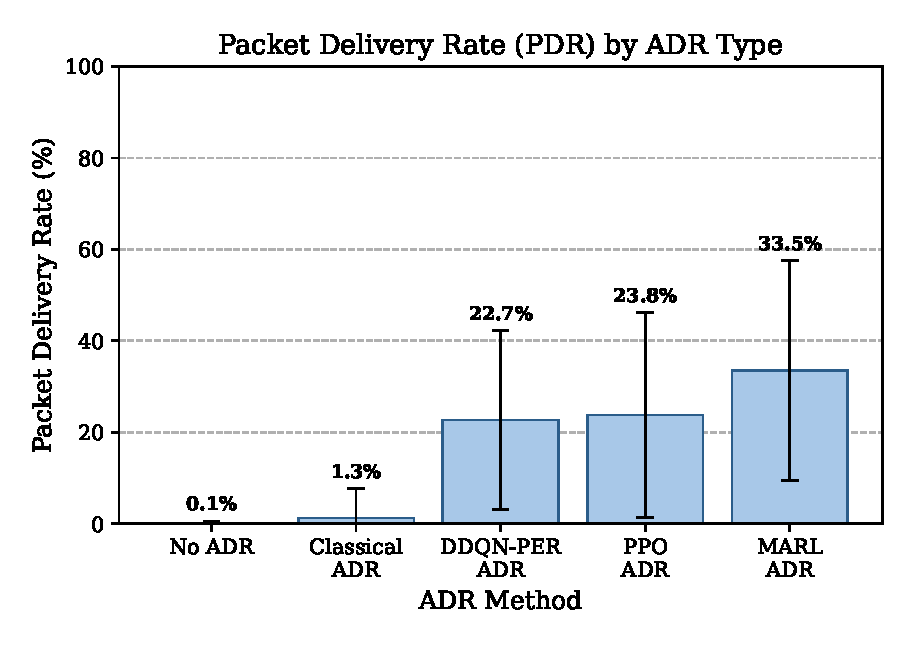
\includegraphics[width=\textwidth]{pdr_by_adr_type_afe.eps}
        \caption{PDR at 100 devices}
    \end{subfigure}
    \hfill
    \begin{subfigure}{0.48\columnwidth}
        \centering
        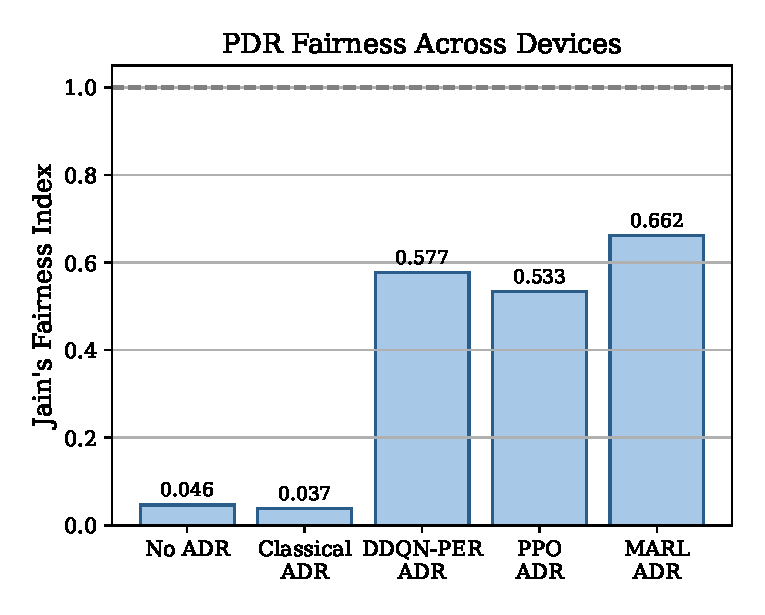
\includegraphics[width=\textwidth]{jains_fairness_afe.eps}
        \caption{Jain's fairness at 100 devices}
    \end{subfigure}
    \caption{Scalability: 100 device, 500~m radius. MARL maintain highest PDR and fairness.}
    \label{fig:scalability}
\end{figure}

Table~\ref{tab:fairness} show that MARL consistently achieve highest Jain's fairness index, meaning it distribute resource more equitably across device. At 100 device, MARL fairness (0.662) is 58\% higher than DQN (0.418).

\begin{table}[t]
\centering
\caption{Jain's fairness index comparison}
\label{tab:fairness}
\footnotesize
\begin{tabular}{@{}lccc@{}}
\toprule
\textbf{Scenario} & \textbf{DQN} & \textbf{PPO} & \textbf{MARL} \\
\midrule
100 dev, 500~m  & 0.418 & 0.434 & \textbf{0.662} \\
200 dev, 500~m  & 0.313 & 0.301 & \textbf{0.547} \\
150 dev, 500~s  & 0.485 & 0.471 & \textbf{0.572} \\
\bottomrule
\end{tabular}
\end{table}

\subsection{Convergence Behavior}

In Experiment 9, we test with only 500~s simulation ($\sim$16 packet per device) to evaluate how quickly agent adapt from random initialization. Even with such limited data, MARL reach 34.96\% PDR where classical ADR manage only 1.05\%. The rapid adaptation is due to heuristic warm-starting: each device initial SF and TP are set based on distance to the gateway, channel are distributed round-robin ($c_i = i \bmod 8$), and an SNR-based ceiling prevent unnecessary SF increase. These engineering heuristic provide a strong initial configuration that the RL agent refine through experience.

Importantly, the dense LoRaWAN optimization is a \textit{continuous, non-stationary game}: as each agent adapt its parameter, the interference landscape change for all others, preventing convergence to a fixed policy. Rather than ``solving'' the problem, agents continuously co-adapt, and the system exhibit dynamic equilibrium where PDR stabilize around a mean with ongoing fluctuation.

Fig.~\ref{fig:convergence} show the PDR convergence at 100 device (Exp~7B), illustrating how MARL agent collectively reach higher PDR over time while single-agent method plateau at lower level.

\begin{figure}[t]
    \centering
    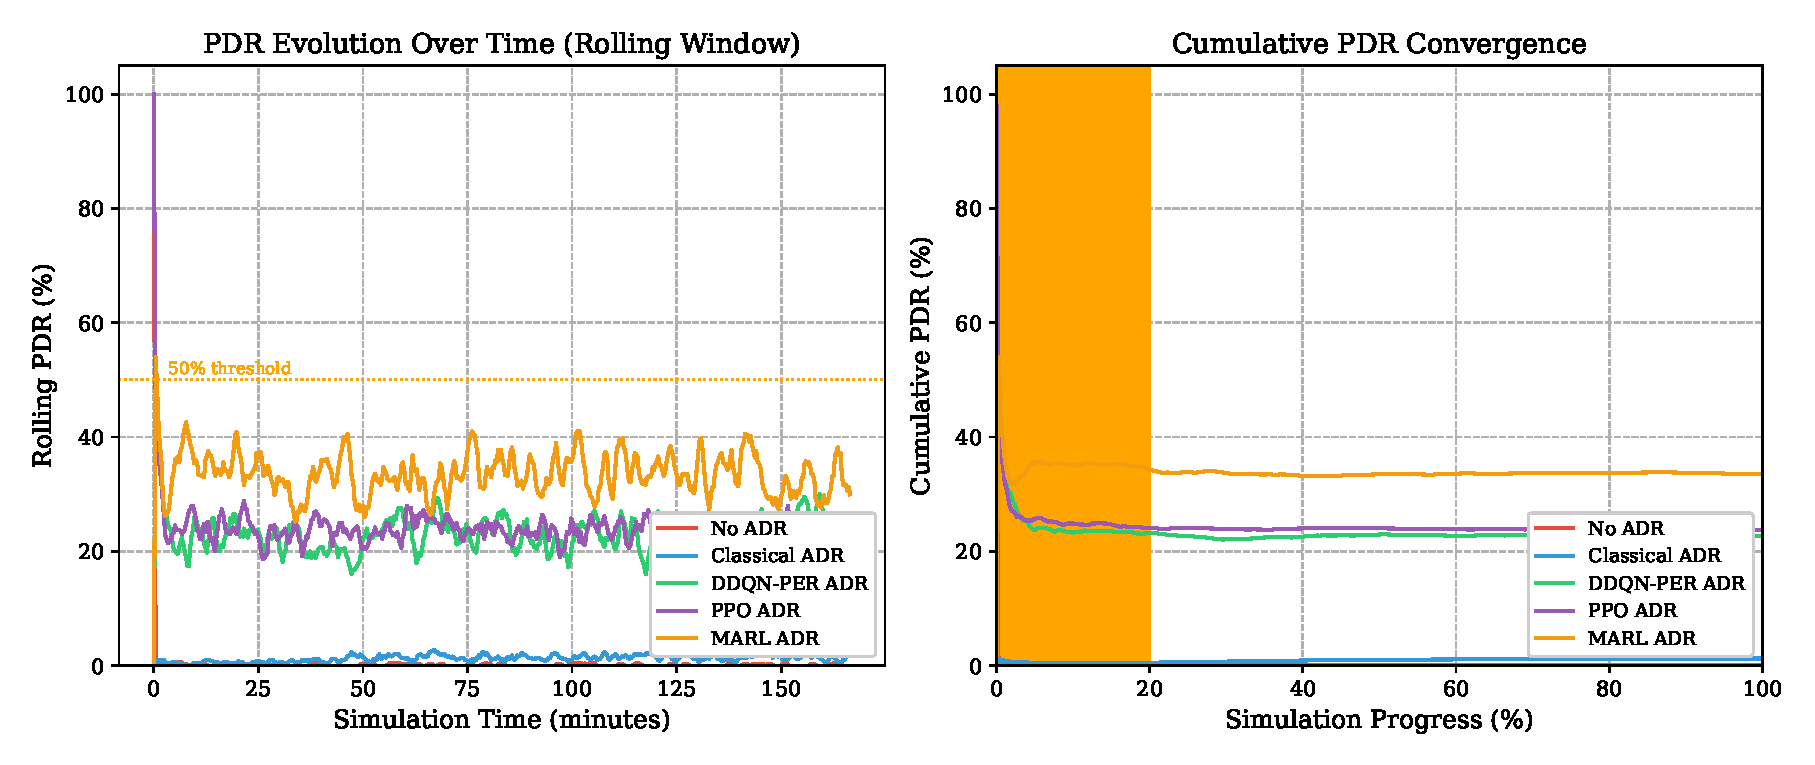
\includegraphics[width=\columnwidth]{pdr_convergence_afe.eps}
    \caption{PDR convergence over time for 100 device, 500~m radius (Exp~7B). MARL achieve higher and more stable PDR through coordination.}
    \label{fig:convergence}
\end{figure}

\subsection{Energy Efficiency}

Table~\ref{tab:energy} compare energy consumption for the ultimate game scenario. MARL and PPO maintain energy comparable to No ADR while delivering $>$99\% of packet. DQN consume 6$\times$ more energy because without coordination, it compensate for collision by increasing SF and TP aggressively. Fig.~\ref{fig:energy} visualize this disparity.

\begin{table}[t]
\centering
\caption{Energy (mJ) for Exp 5: 20 dev, 100~m}
\label{tab:energy}
\footnotesize
\begin{tabular}{@{}lcc@{}}
\toprule
\textbf{Method} & \textbf{Mean Energy (mJ)} & \textbf{PDR (\%)} \\
\midrule
No ADR       & 79,500  & 31.94 \\
Classical    & 74,301  & 42.07 \\
DQN-PER      & 487,277 & 99.24 \\
PPO          & 77,443  & 99.33 \\
\textbf{MARL} & \textbf{79,484} & \textbf{99.63} \\
\bottomrule
\end{tabular}
\end{table}

At extreme scale (100 device, 500~m), MARL energy (36,913~mJ) is the lowest of all method---even lower than classical ADR (68,913~mJ). This is because MARL agent collectively learn to use the lowest possible SF and TP through coordination.

\begin{figure}[t]
    \centering
    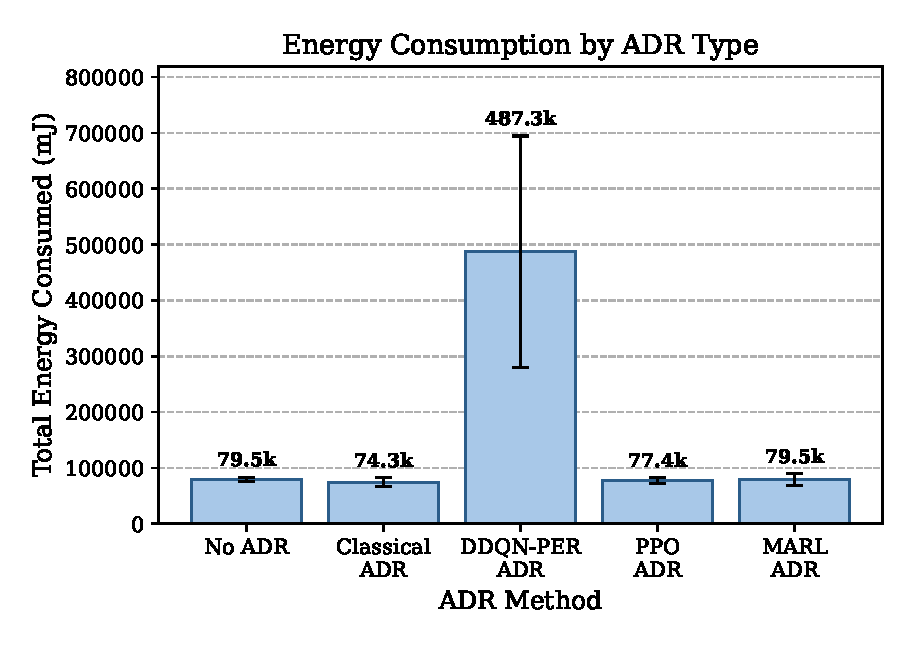
\includegraphics[width=\columnwidth]{energy_by_adr_type_82a.eps}
    \caption{Energy consumption comparison for Exp~5 (20 device, 100~m). DQN-PER consume 6$\times$ more energy than MARL due to aggressive SF/TP increase without coordination.}
    \label{fig:energy}
\end{figure}

\subsection{Physical Testbed Validation}

We validate the approach with a physical testbed consisting of 3 ESP32 microcontroller with SX1278 LoRa transceiver module, an STM32-based Arduino Portenta H7 gateway, and a PC-based network server. The system successfully run inference of the trained Q-network on ESP32 and update SF/TP via downlink MAC command. This demonstrate that the computational requirement of the RL agent are within the capability of resource-constrained IoT hardware.

% ============================================================================
\section{Discussion}
\label{sec:discussion}
% ============================================================================

Our result reveal several important insight for practical LoRaWAN deployment:

\textbf{Coordination is more important than algorithm complexity.} The performance gap between MARL and single-agent method (DQN, PPO) is primarily driven by the coordination signal, not by the underlying algorithm. Both MARL and DQN use the same Dueling DQN architecture. The simple addition of channel congestion information to the state vector and the coordination-aware action selection policy (Algorithm~\ref{alg:marl}) produce the key improvement.

\textbf{The SF7 congestion paradox.} Classical ADR follow the rule: ``if SNR is good, use SF7.'' In dense deployment, this cause all close-range device to converge to SF7, creating massive collision on a single logical channel. MARL agent learn to spread device across physical channel even when all could technically use SF7, effectively solving the frequency allocation problem through distributed learning.

\textbf{Scalability limit exist.} At 200 device, even MARL deliver only 17.64\% PDR. This represent a fundamental capacity limit of single-gateway LoRaWAN with 8 channel. Beyond this point, gateway densification or non-ALOHA MAC protocol would be needed.

\textbf{Practical deployment feasibility.} Heuristic warm-starting enable meaningful adaptation within $\sim$16 packet (Exp~9), as agent benefit from distance-based SF/TP initialization and round-robin channel distribution, eliminating the concern about long warm-up period in real deployment. The network server maintain the channel map and provide coordination signal through standard downlink MAC command, requiring no modification to the LoRaWAN protocol stack.

% ============================================================================
\section{Related Work}
\label{sec:related}
% ============================================================================

ADR optimization in LoRaWAN have been approached from multiple direction. Cuomo et al. \cite{cuomo2017explora} propose EXPLoRa that assign SF based on equalization strategy, but lack adaptivity to dynamic condition. Reynders et al. \cite{reynders2017power} demonstrate that joint SF and TP optimization improve energy efficiency but use exhaustive search. Farhad et al. \cite{farhad2021deep} apply deep learning to predict optimal ADR parameter from network state, showing improvement over classical ADR, but the supervised approach cannot adapt to unseen condition. 

In RL-based approach, Ta et al. \cite{ta2023enhanced} propose enhanced RL for transmission parameter selection and demonstrate PDR and energy optimization, but for a single device in isolation---ignoring the competitive multi-agent dynamics that dominate dense networks. Moy et al. \cite{moy2024energy} apply RL to subterranean LoRaWAN in satellite scenario, showing benefit of adaptive parameter selection, but the single-gateway subterranean setup with few device bear little resemblance to dense surface deployment. Yazid et al. \cite{yazid2022rl} formulate parameter selection as an MDP and validate with tabular Q-learning on 10 stationary device with fixed interference, providing no evidence of scalability or robustness under dynamic condition. Abdelfadeel et al.~\cite{abdelfadeel2020machine} propose a fair ADR based on centralized SF equalization heuristic, but this require full global state knowledge and cannot react to time-varying interference from WiFi or LTE source.

Multi-agent approach in wireless network have been studied \cite{littman1994markov, luong2019applications}, but application to LoRaWAN ADR with explicit channel coordination remain unexplored. Our work is the first to evaluate MARL-based ADR at scale (up to 200 device) with comprehensive fairness and convergence analysis.

% ============================================================================
\section{Conclusion}
\label{sec:conclusion}
% ============================================================================

We present a Multi-Agent Reinforcement Learning approach for ADR optimization in dense LoRaWAN network. By extending Independent Q-Learning with coordination signal for channel-aware collision avoidance, MARL achieve up to 99.63\% PDR in scenario where classical ADR deliver only 42\%, while maintaining comparable energy consumption. The scalability analysis across 10 to 200 device show that MARL degrade more gracefully with 58\% higher fairness than single-agent method. Heuristic warm-starting enable meaningful adaptation within $\sim$16 packet, and physical testbed validation confirm deployment feasibility on resource-constrained IoT device.

Future work will explore dynamic coordination signal beyond channel congestion, such as SF distribution awareness, and investigate the scalability with multiple gateway in heterogeneous network deployment.

% ============================================================================
% REFERENCES
% ============================================================================

\balance
\begin{thebibliography}{20}

\bibitem{Raza17}
U.~Raza, P.~Kulkarni, and M.~Sooriyabandara, ``Low power wide area networks: An overview,'' \textit{IEEE Commun. Surveys Tuts.}, vol.~19, no.~2, pp.~855--873, 2017.

\bibitem{augustin2016study}
A.~Augustin, J.~Yi, T.~Clausen, and W.~M. Townsley, ``A study of LoRa: Long range \& low power networks for the Internet of Things,'' \textit{Sensors}, vol.~16, no.~9, p.~1466, 2016.

\bibitem{georgiou2017low}
O.~Georgiou and U.~Raza, ``Low power wide area network analysis: Can LoRa scale?'' \textit{IEEE Wireless Commun. Lett.}, vol.~6, no.~2, pp.~162--165, 2017.

\bibitem{bor2016lora}
M.~C. Bor, U.~Roedig, T.~Voigt, and J.~M. Alonso, ``Do LoRa low-power wide-area networks scale?'' in \textit{Proc. ACM MSWiM}, 2016, pp.~59--67.

\bibitem{bankov2016mathematical}
D.~Bankov, E.~Khorov, and A.~Lyakhov, ``On the limits of LoRaWAN channel access,'' in \textit{Proc. IEEE ICESS}, 2016, pp.~10--14.

\bibitem{slabicki2018adaptive}
M.~Slabicki, G.~Premsankar, and M.~Di Francesco, ``Adaptive configuration of LoRa networks for dense IoT deployments,'' in \textit{Proc. IEEE/IFIP NOMS}, 2018, pp.~1--9.

\bibitem{farhad2021deep}
A.~Farhad, D.-H. Kim, S.~Subedi, and J.-Y. Pyun, ``A deep learning-based adaptive data rate algorithm for LoRaWAN networks,'' \textit{Comput., Mater. Continua}, vol.~69, no.~3, pp.~3767--3781, 2021.

\bibitem{ta2023enhanced}
D.-T. Ta, K.~Nguyen, and S.~Fdida, ``Enhanced reinforcement learning algorithm based-transmission parameter selection for optimization of energy consumption and packet delivery ratio in LoRa wireless networks,'' \textit{Comput. Netw.}, vol.~226, p.~109681, 2023.

\bibitem{moy2024energy}
C.~Moy, M.~Music, and A.~Music, ``Energy efficiency optimization for subterranean LoRaWAN using a reinforcement learning approach: A direct-to-satellite scenario,'' \textit{IEEE Access}, vol.~12, pp.~45312--45326, 2024.

\bibitem{yazid2022rl}
Y.~Yazid, I.~Ez-Zazi, A.~Guerrero-Gonz\'alez, A.~El~Oualkadi, and M.~Arioua, ``A reinforcement learning based transmission parameter selection and energy management for long range Internet of Things,'' \textit{Sensors}, vol.~22, no.~15, p.~5662, 2022.

\bibitem{abdelfadeel2020machine}
K.~Q. Abdelfadeel, V.~Cionca, and D.~Pesch, ``Fair adaptive data rate allocation in LoRaWAN,'' in \textit{Proc. IEEE WoWMoM}, 2020, pp.~1--10.

\bibitem{cuomo2017explora}
F.~Cuomo, M.~Campo, A.~Caponi, G.~Bianchi, G.~Rossini, and P.~Luvisotto, ``EXPLoRa: Extending the performance of LoRa by suitable spreading factor allocations,'' in \textit{Proc. IEEE WiMob}, 2017, pp.~1--8.

\bibitem{reynders2017power}
B.~Reynders, W.~Meert, and S.~Pollin, ``Power and spreading factor control in low power wide area networks,'' in \textit{Proc. IEEE ICC}, 2017, pp.~1--6.

\bibitem{reynders2018improving}
B.~Reynders, Q.~Wang, P.~Tuset-Peiro, X.~Vilajosana, and S.~Pollin, ``Improving reliability and scalability of LoRaWANs through lightweight scheduling,'' \textit{IEEE Internet Things J.}, vol.~5, no.~3, pp.~1830--1842, 2018.

\bibitem{hosseinzadeh2020empirical}
S.~Hosseinzadeh, M.~Almoathen, H.~Larijani, and K.~Curtis, ``A neural network propagation model for LoRaWAN and critical analysis with real-world measurements,'' \textit{Big Data Cognitive Computing}, vol.~4, no.~3, p.~7, 2020.

\bibitem{semtech_sx1278}
Semtech Corporation, ``SX1276/77/78/79 -- 137~MHz to 1020~MHz low power long range transceiver,'' datasheet, Rev.~7, 2020.

\bibitem{semtech_adr}
Semtech Corporation, ``LoRaWAN adaptive data rate,'' LoRa Developer Portal, 2021.

\bibitem{wang2016dueling}
Z.~Wang, T.~Schaul, M.~Hessel, H.~Van~Hasselt, M.~Lanctot, and N.~De~Freitas, ``Dueling network architectures for deep reinforcement learning,'' in \textit{Proc. ICML}, 2016, pp.~1995--2003.

\bibitem{schaul2016per}
T.~Schaul, J.~Quan, I.~Antonoglou, and D.~Silver, ``Prioritized experience replay,'' in \textit{Proc. ICLR}, 2016.

\bibitem{van2016deep}
H.~Van~Hasselt, A.~Guez, and D.~Silver, ``Deep reinforcement learning with double Q-learning,'' in \textit{Proc. AAAI}, 2016, pp.~2094--2100.

\bibitem{schulman2017ppo}
J.~Schulman, F.~Wolski, P.~Dhariwal, A.~Radford, and O.~Klimov, ``Proximal policy optimization algorithms,'' \textit{arXiv preprint arXiv:1707.06347}, 2017.

\bibitem{littman1994markov}
M.~L. Littman, ``Markov games as a framework for multi-agent reinforcement learning,'' in \textit{Proc. ICML}, 1994, pp.~157--163.

\bibitem{luong2019applications}
N.~C. Luong, D.~T. Hoang, S.~Gong, D.~Niyato, P.~Wang, Y.-C. Liang, and D.~I. Kim, ``Applications of deep reinforcement learning in communications and networking: A survey,'' \textit{IEEE Commun. Surveys Tuts.}, vol.~21, no.~4, pp.~3133--3174, 2019.

\bibitem{riley2010ns3}
G.~F. Riley and T.~R. Henderson, ``The ns-3 network simulator,'' in \textit{Modeling and Tools for Network Simulation}, Springer, 2010, pp.~15--34.

\end{thebibliography}

\end{document}
